\documentclass[12pt,a4paper]{article}
\usepackage{blindtext}\usepackage{accsupp}
% Packages for various functionalities
\usepackage{amssymb}
\usepackage{wasysym}
\usepackage[utf8]{inputenc}
\usepackage{physics} % Assuming you resolved the package conflicts
\usepackage{anyfontsize}
\usepackage{amsmath,mathtools}
\usepackage[margin=0.65in]{geometry}
\usepackage{xcolor}
\usepackage{fancyhdr}
\usepackage{amsfonts}
\usepackage[euler]{textgreek}
\usepackage{chemformula}
\usepackage{titlesec} % For customizing section heading sizes
\usepackage{indentfirst} % For indenting the first paragraph of each section
\usepackage[hidelinks]{hyperref} 
\usepackage{tabularx}
\usepackage{graphicx}
\usepackage{array}
\usepackage{listings}
\usepackage{xcolor}
\usepackage{pdfpages}
\usepackage{booktabs}
\usepackage{enumitem}
% Custom headers and footers using fancyhdr package
\pagestyle{fancy}
\fancyhead[L]{\footnotesize Institute of Polytechique of Grenoble}
\fancyhead[R]{\footnotesize New Sustainable Technoglogies}
\fancyhead[C]{\footnotesize 2024 - 2025}
\renewcommand{\headrulewidth}{0.5pt}
\renewcommand{\footrulewidth}{0.5pt}
\fancyfoot[R]{\textcolor{black}{\footnotesize SARY MONYCHOT \& NIANG BORA}}
\fancyfoot[L]{\footnotesize}

% Set up table formatting
\setlength{\arrayrulewidth}{0.5mm}
\setlength{\tabcolsep}{15pt}
\renewcommand{\arraystretch}{0.95}

% Custom command for electron representation

\newcolumntype{C}{>{\centering\arraybackslash}X}
% Customize section heading sizes
\titleformat{\section}{\normalfont\large\Roman{\bfseries}}{\thesection}{1em}{}
\titleformat{\subsection}{\normalfont\normalsize\bfseries}{\thesubsection}{0.75em}{}
\titleformat{\subsubsection}{\normalfont\normalsize\bfseries}{\thesubsubsection}{0.5em}{}

% Customize equation numbering to include section number
\numberwithin{equation}{section}
\lstset{ 
	language=Python,                 % the language of the code
	basicstyle=\ttfamily\footnotesize, % the size of the fonts that are used for the code
	numbers=left,                   % where to put the line-numbers
	numberstyle=\tiny\color{gray},  % the style that is used for the line-numbers
	stepnumber=1,                   % the step between two line-numbers. If it's 1, each line will be numbered
	numbersep=5pt,                  % how far the line-numbers are from the code
	backgroundcolor=\color{white},      % choose the background color. You must add \usepackage{color}
	showspaces=false,               % show spaces adding particular underscores
	showstringspaces=false,         % underline spaces within strings
	showtabs=false,                 % show tabs within strings adding particular underscores
	frame=single,                   % adds a frame around the code
	rulecolor=\color{black},        % if not set, the frame-color may be changed on line-breaks within not-black text (e.g. comments (green here))
	tabsize=4,                      % sets default tabsize to 2 spaces
	captionpos=b,                   % sets the caption-position to bottom
	breaklines=true,                % sets automatic line breaking
	breakatwhitespace=false,        % sets if automatic breaks should only happen at whitespace
	keywordstyle=\color{blue},      % keyword style
	commentstyle=\color{green},   % comment style
	stringstyle=\color{red},      % string literal style
}

\begin{document}
	\title{\textbf{PEM Fuel Cell system analysis }}
	\author{SARY Monychot \& NIANG Bora }
	\date{\today}
	\maketitle
		% Table of Contents
	\tableofcontents
% =============================================================	
		\newpage
%% =======================================1 . =========================================
	% Sections and Subsections
	\section{\underline{Calculation of the power demand inside the vechicle}}
	\begin{itemize}
	 \item The specification of the vehicle are the following:
	
	\begin{itemize}
		\item  Weight $M = 2000 kg$
		\item Front area $A = 2.25  m^2$
		\item Drag coefficient (or air penetration coefficient) $C = 0.29$ 
		\item Rolling Resistance coefficient $C_r = 0.0115$
		
	\end{itemize}
	
	\item The efforts applied on the vehicle in the rolling direction have to following expression:
	
	\begin{itemize}
		\item Air penetration : 
		\begin{equation}
				F = \frac{1}{2}\rho_{air}v^2CA  \label{eq1}
		\end{equation} with $\rho_{air} = 1.2    kg/m^3$
		\item Rolling resistance :	
		\begin{equation}
			 F = MgC_r\cos{\alpha} \label{eq2}
		\end{equation}with $g = 9.81 m/s^2$ and $\alpha$ the slope angle
		\item Climbing or descent : 
		\begin{equation}
			F = Mg\sin{\alpha} \label{eq3}
		\end{equation} 
		
	\end{itemize}
	\end{itemize}
	
	
%% ======================================= a . =========================================	

	\subsection{Calculate and plot the instant power provided by the vechicle powertrain for the road cycles " WLTC " }
	
	$\star$ Consider a flat road $(\alpha = 0)$
	\begin{figure}[htbp]
		\centering
		\begin{tabular}{c @{\qquad} c}
			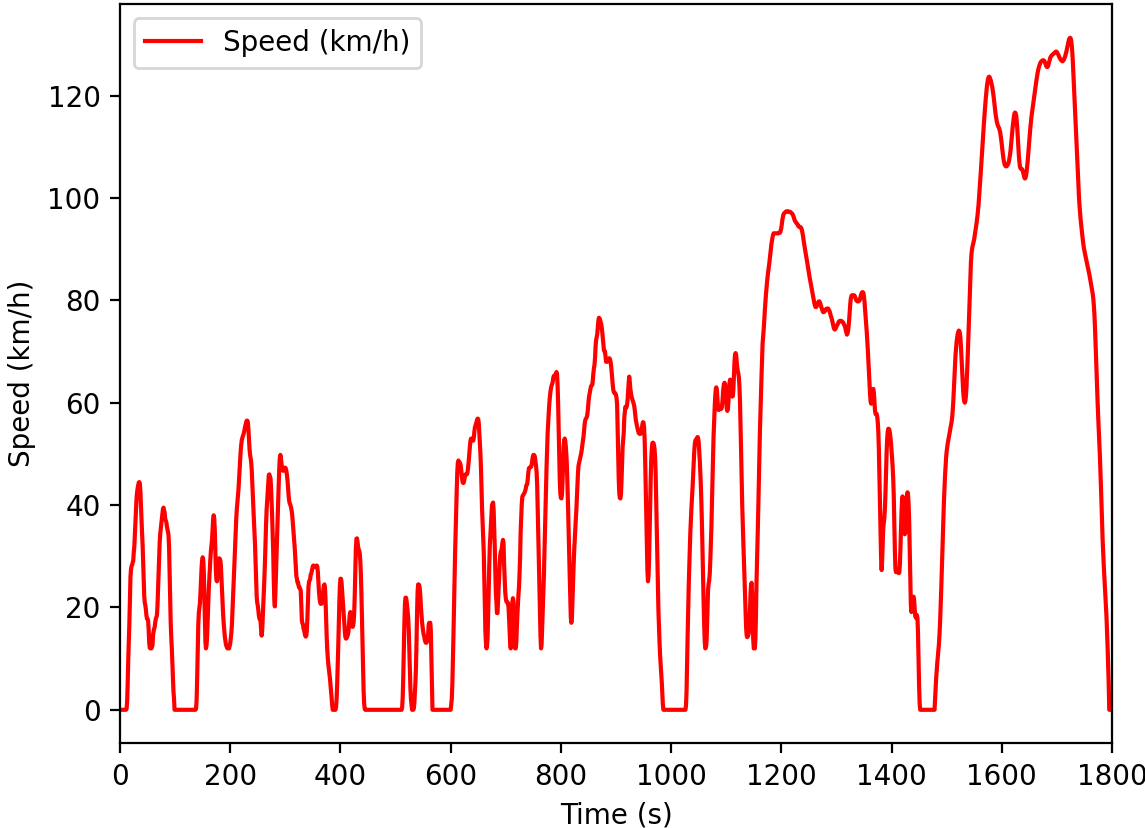
\includegraphics[width=0.48\linewidth]{E:/07. Master_Degree_ITC+UGA/02. ENES3_SGB_UGA/02. New Technology/PEMFC/Speed_1.png} &
			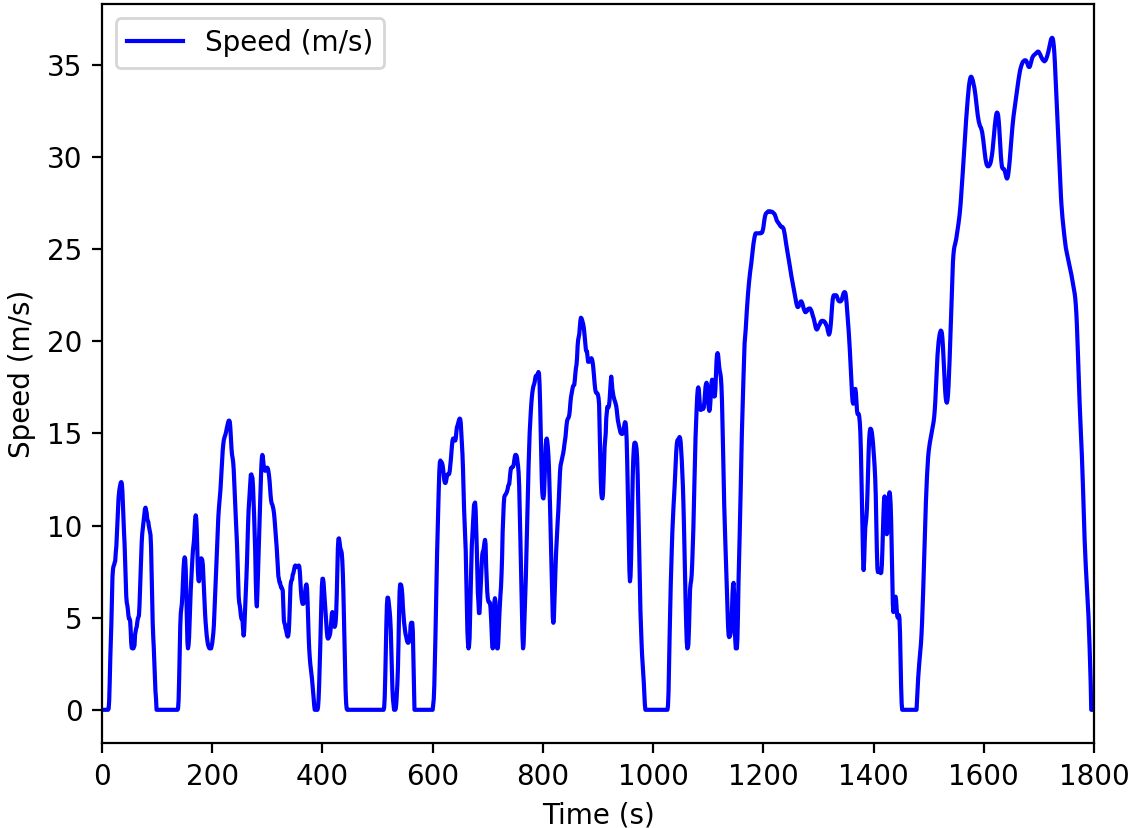
\includegraphics[width=0.48\linewidth]{E:/07. Master_Degree_ITC+UGA/02. ENES3_SGB_UGA/02. New Technology/PEMFC/Speed ms-1_1.png} \\
			
			\small (a) Speed Profile in km/h & \small (b) Speed Profile in m/s
		\end{tabular}
		
		\caption{\small Graph of the Speed Profile in km/h and Speed in m/s}
		\label{1}
	\end{figure}

%% ========================================================================================================
	\subsubsection{Calculation}
	
	To calculate the \textbf{Instant Power}, we need to study of the \textit{force} that have action on the car. By using second Newton's law with the Figure (\ref{2}) shown below, we can assume that there are 4 forces that have action on thecar while driving.
	
	\begin{figure}[h]
		\centering 
		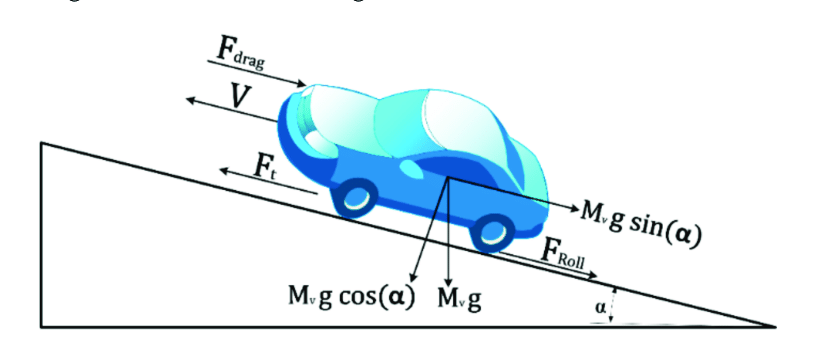
\includegraphics[width=0.7\linewidth]{E:/07. Master_Degree_ITC+UGA/02. ENES3_SGB_UGA/02. New Technology/PEMFC/2.png}
		\caption{\small {Speed (km/h) of the vechicle powertrain by time (s)}}
		\label{2}
	\end{figure}



	\begin{itemize}
		\item The first force is to make the car move in direction. It called the force from motor or machine of the car ($F_{motor}$)
		\item The second force is the rolling force from the car wheels. It called \textbf{Rolling Resistance} ($F_{rolling}$)
		\item The third force is the climbing or descent force ($F_{climb}$)
		\item The fourth force is the force from the air friction. we can called it Air penetration ($F_{air}$).
	\end{itemize}


	Using second Newton's law, we can written :
	\begin{equation}
		\overrightarrow{F}_{motor} - \overrightarrow{F}_{rolling} -\overrightarrow{F}_{climb} - \overrightarrow{F}_{air} = m\overrightarrow{a}
		\label{eq4}
	\end{equation}
	\begin{equation}
		\overrightarrow{F}_{motor} = \overrightarrow{F}_{rolling} + \overrightarrow{F}_{climb} + \overrightarrow{F}_{air} + m\overrightarrow{a}
		\label{eq5}
	\end{equation}

	since $a$ is the acceleration of the vechical in time $t$, as we written : 
	\begin{equation}
		\overrightarrow{a} = \derivative{\overrightarrow{v}}{t} = \frac{\Delta v}{\Delta t}
		\label{eq6}
	\end{equation}

	By using Equation (\ref{eq6}), we can get the result of acceleration on the Figure (\ref{3})
	\begin{figure}[h]
		\centering 
		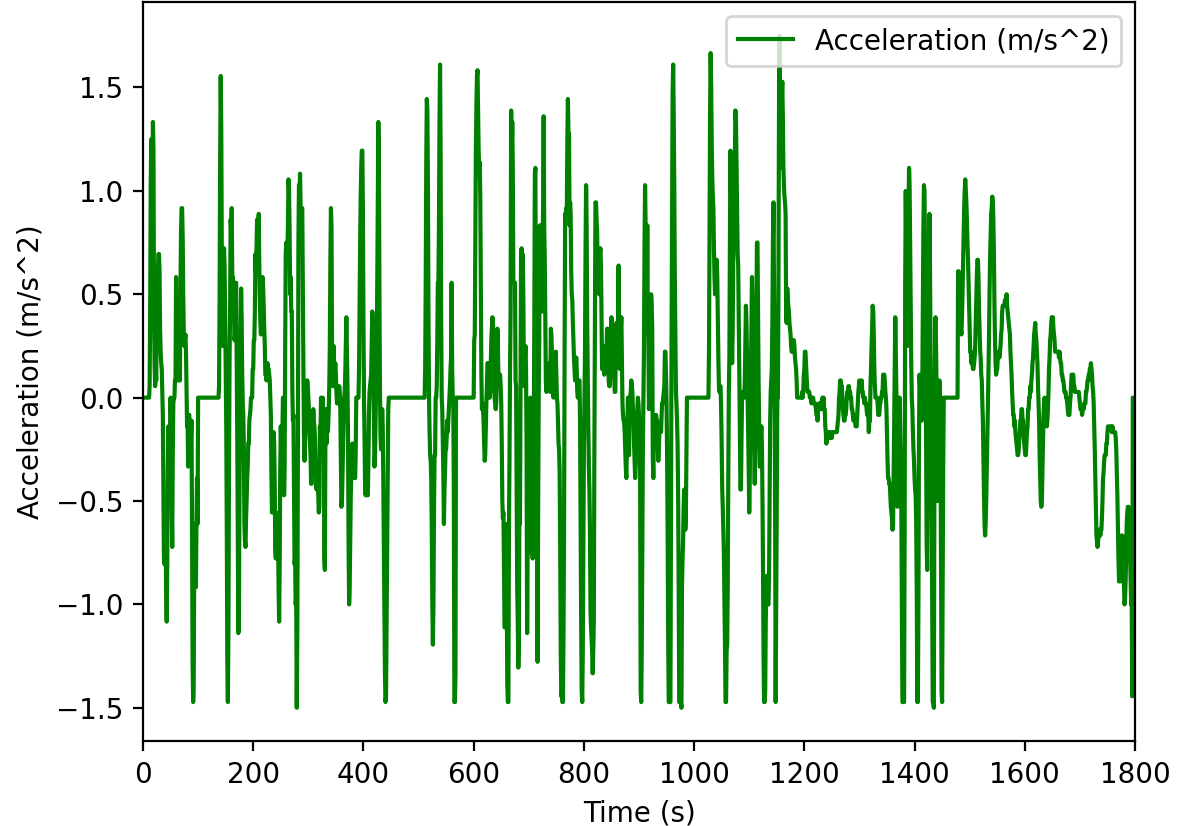
\includegraphics[width=0.65\linewidth]{E:/07. Master_Degree_ITC+UGA/02. ENES3_SGB_UGA/02. New Technology/PEMFC/Acceleration_1.png}
		\caption{\small {Acceleration $(m/s^2)$ of the vechicle powertrain by time (s)}}
		\label{3}
	\end{figure}

	According to the graph, it shown that the vechical did not have the stable speed drive on the. At the some time ($t$), the vechical increasing the speed immediately. In contrast, at some time ($t$), the vechical reducing the speed quickly as shown in the Figure (\ref{3}).

	\begin{itemize}[label=-]
		\item For calculate $F_{air}$ by using Equation (\ref{eq1}) , we got :
			\begin{equation}
				F_{air} = \frac{1}{2}\rho_{air}v^2CA = \frac{1}{2}\times1.2\times 	v^2_{m/s}_{,t}\times0.29\times 2.25 \label{eq7}
			\end{equation}
			In this section, to calculate $F_{air}$ we need to get the speed in each time $t$ in $m/s^2$ to analyze in the Equation (\ref{eq7})
			By using the Equation (\ref{eq1}), we got the result of the force air penetration by shown in below graph.
		\item For calculate $F_{rolling}$, we will be using the Equation (\ref{eq2}), we got :
			\begin{equation}
				F_{rolling} = MgC_r\cos(\alpha) = 2000kg\times9.81m/s^2\times0.0115\times\cos(0^\circ) = \textbf{225.630} \label{eq8}
			\end{equation}
			For this force, it will be constant in time $(t)$ becuase there is not any parameter in the Equation (\ref{eq8}) will change in which time.
			
			
		\item For calculate $F_{climb}$, we will use Equation (\ref{eq4}) then we got:
		
			\begin{equation}
				F = Mg\sin(\alpha) = 2000kg \times 9.81m/s^2 \times \sin(0^\circ) = 0 \label{eq9}
			\end{equation}		
	\end{itemize}

	By using Equation (\ref{eq6}), (\ref{eq7}), (\ref{eq8}) and (\ref{eq9}) substitution into Equation (\ref{eq5}). The result of total force was shown by the graph in Figure (\ref{4}).
	
	\begin{figure}[htbp]
		\centering
		\begin{tabular}{c @{\qquad} c}
			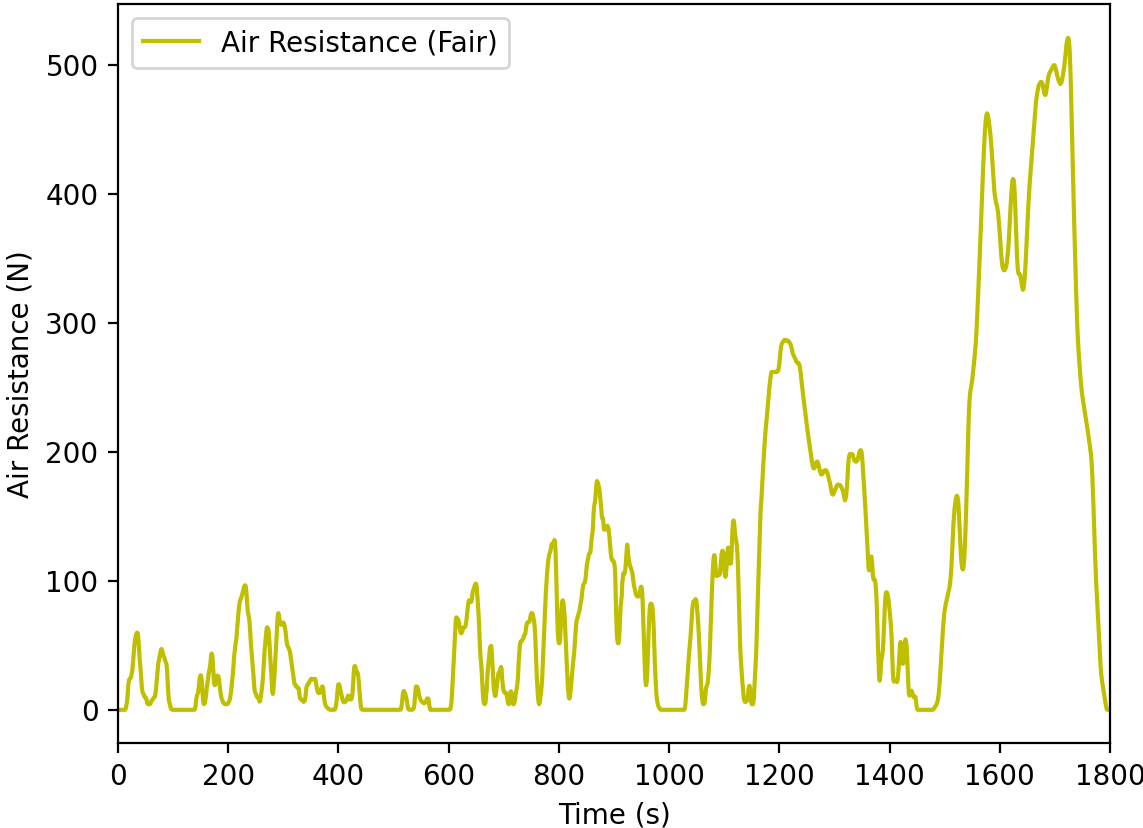
\includegraphics[width=0.48\linewidth]{E:/07. Master_Degree_ITC+UGA/02. ENES3_SGB_UGA/02. New Technology/PEMFC/Fair_1.png} &
			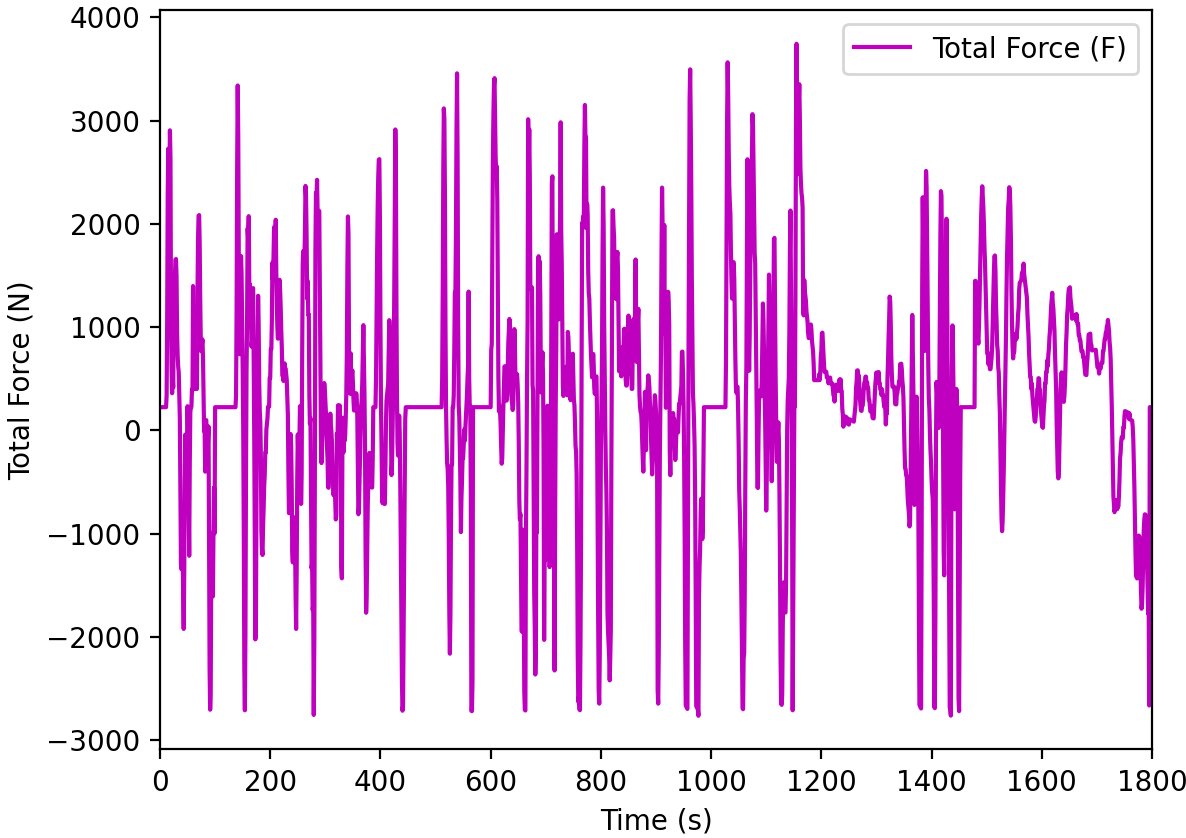
\includegraphics[width=0.48\linewidth]{E:/07. Master_Degree_ITC+UGA/02. ENES3_SGB_UGA/02. New Technology/PEMFC/Total_Force_1.png} \\
			
			\small (a) Force of Air Resistance & \small (b) Total Force
		\end{tabular}
		
		\caption{\small Graph of the  Force of Air Resistance and Total Force}
		\label{4}
	\end{figure}
		
	To calculate Instant power we are using :
	
	\begin{equation}
		P = F \times v \label{eq10}
	\end{equation}	
	
	The result of the instant power calcuation will be show at Figure (\ref{5})b. The instant power of the vechical are depend on two parameter :
	\begin{itemize}
		\item The total force from the vechical action ($N$).
		\item The speed that make the vechical go forward ($m/s$).
	\end{itemize}	                                                                                                                                                                  
	\indent As now, we can write that 
		\begin{equation}
			P_t = F_t \times v_t 
		\end{equation} 
	\newpage
	
	 The result of the instant power will show in the Figure ({\ref{5}).
	 
	 \begin{figure}[h]
	 	\centering 
	 	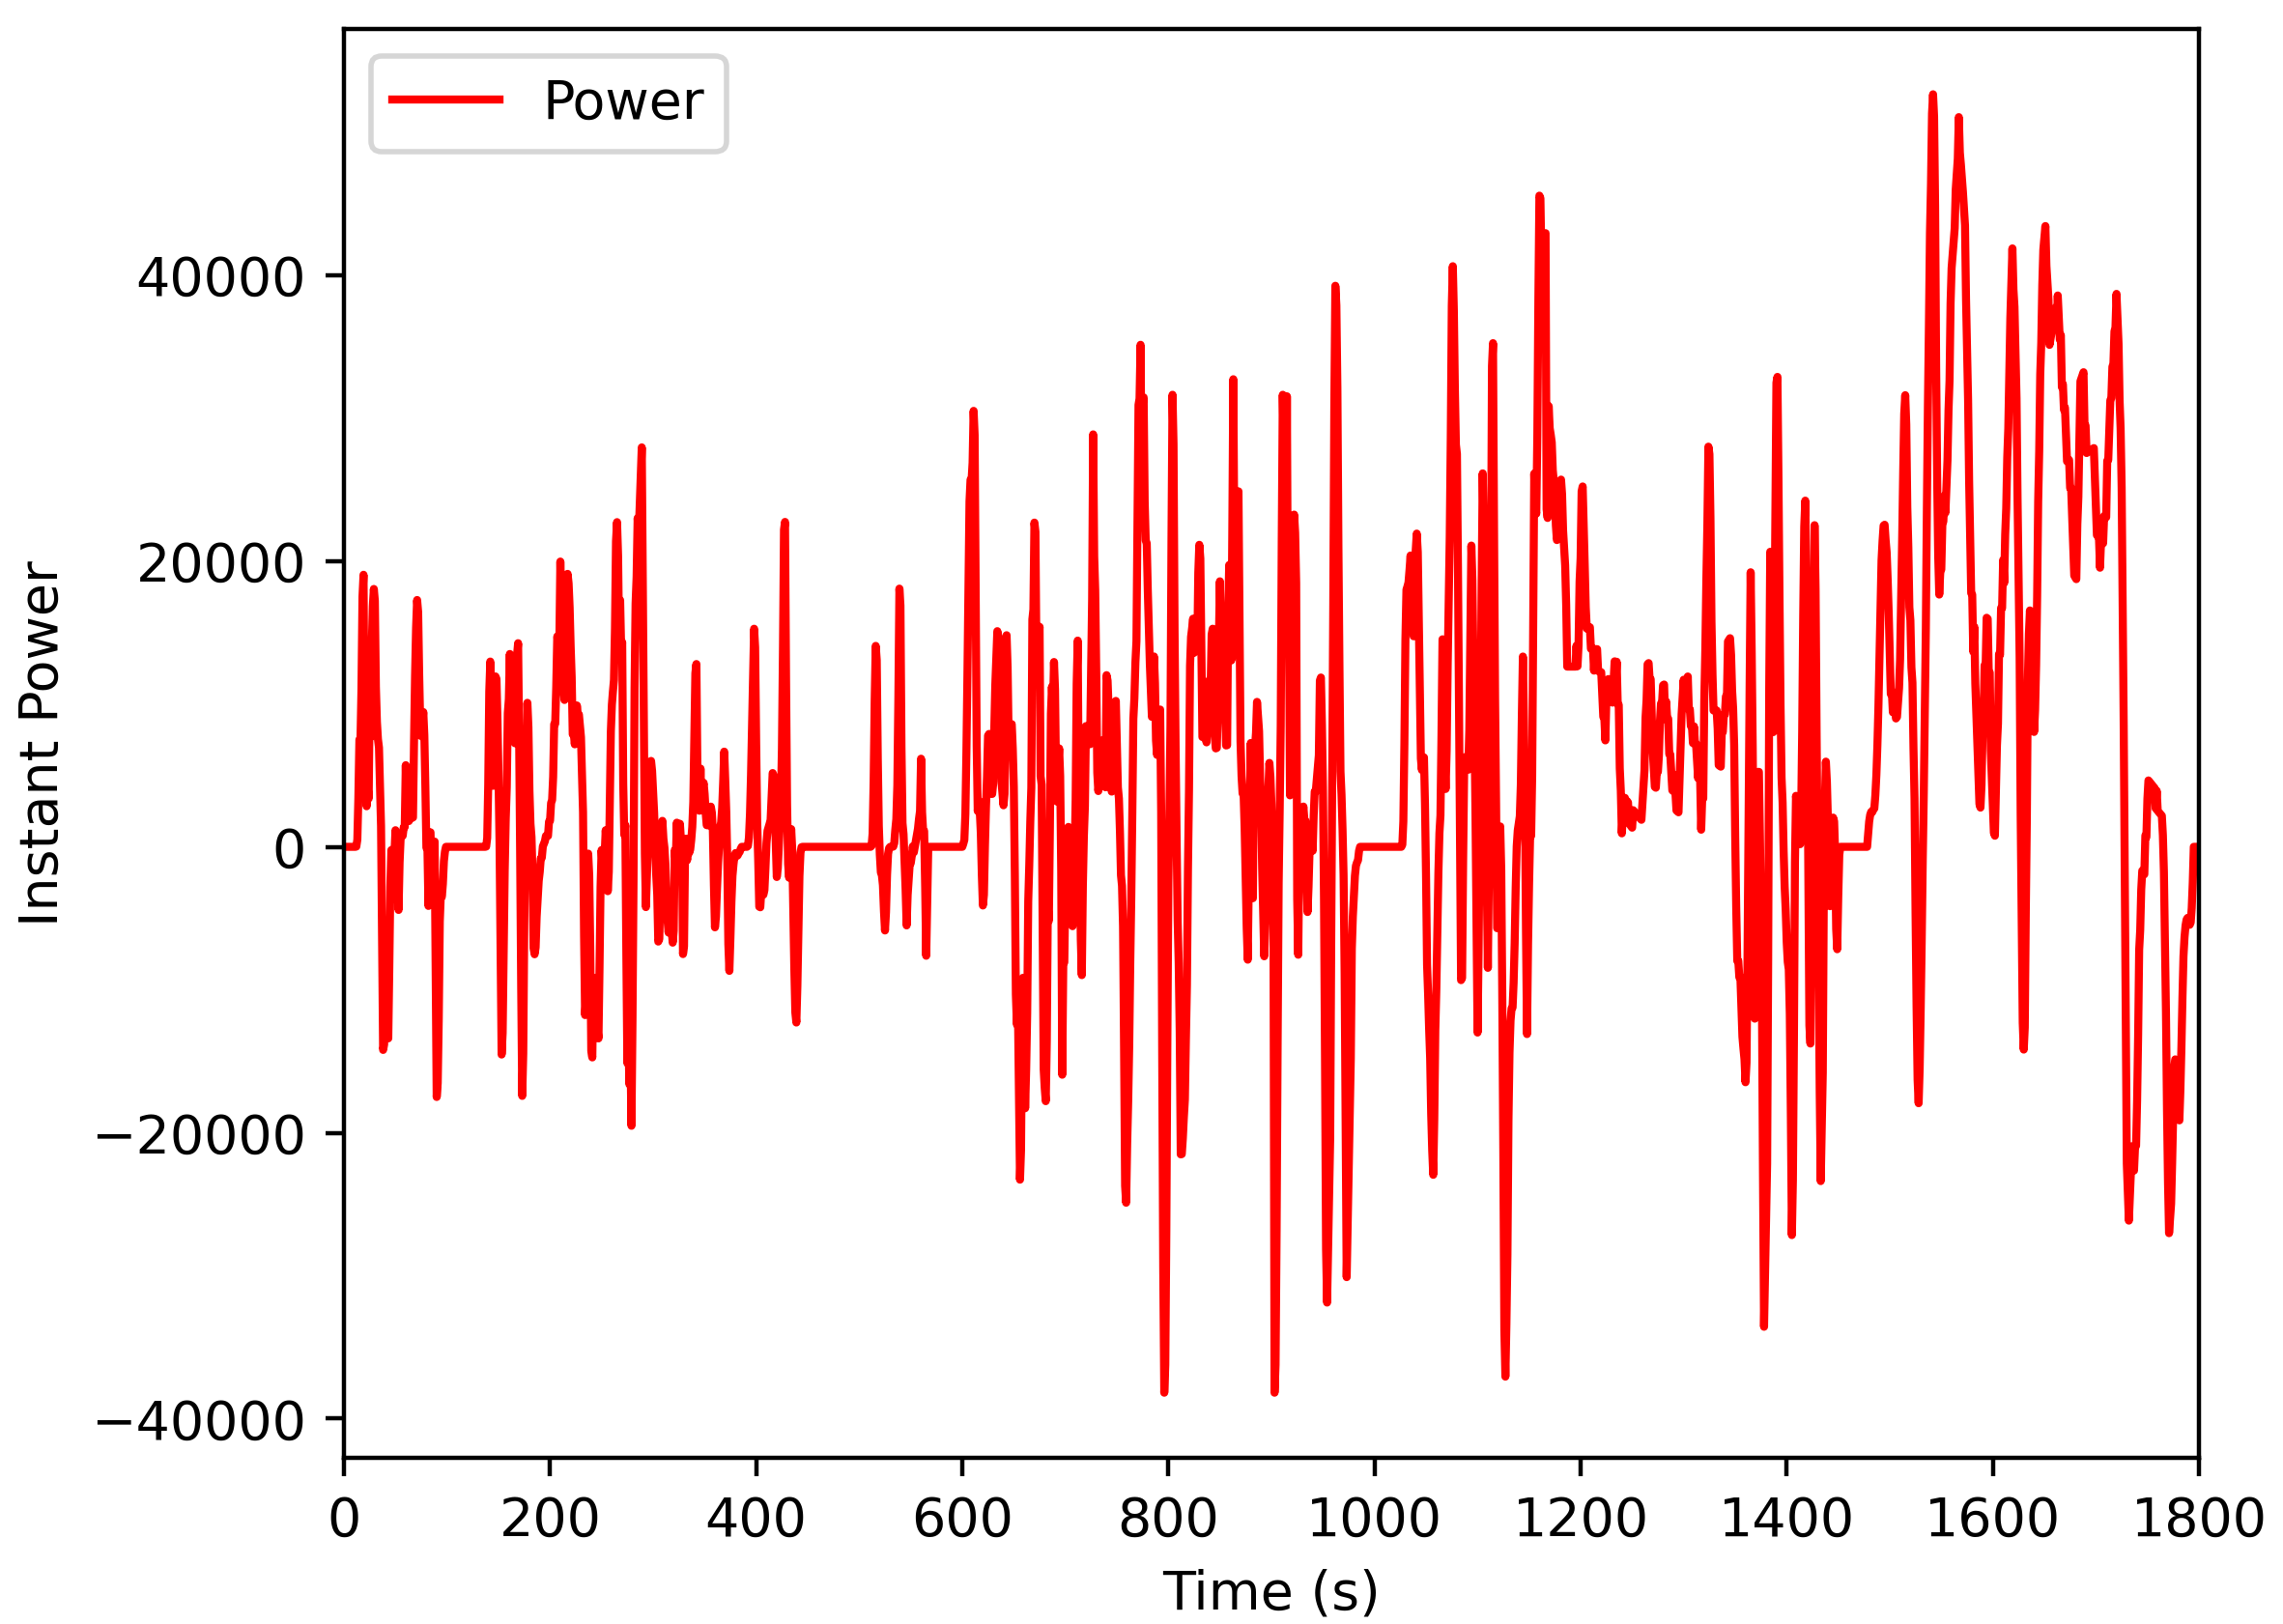
\includegraphics[width=0.7\linewidth]{E:/07. Master_Degree_ITC+UGA/02. ENES3_SGB_UGA/02. New Technology/PEMFC/Power_1.png}
	 	\caption{\small {Instant Power of the Vechicle (W)}}
	 	\label{5}
	 \end{figure}
	
%% ======================================= b . =========================================

	\subsection{Calculate the instant power provide (positive) or received (negative) by the electric hybrid power source. }
	
	The vehicle auxiliaries consume an electrical power of 300W (no air conditioning, minimum consumption of all the equipment of the vehicle: sensor, supervisor,etc.) The DC/DC converter efficiency is assumed constant at 90\% both direction.
	
	\begin{figure}[h]
		\centering 
		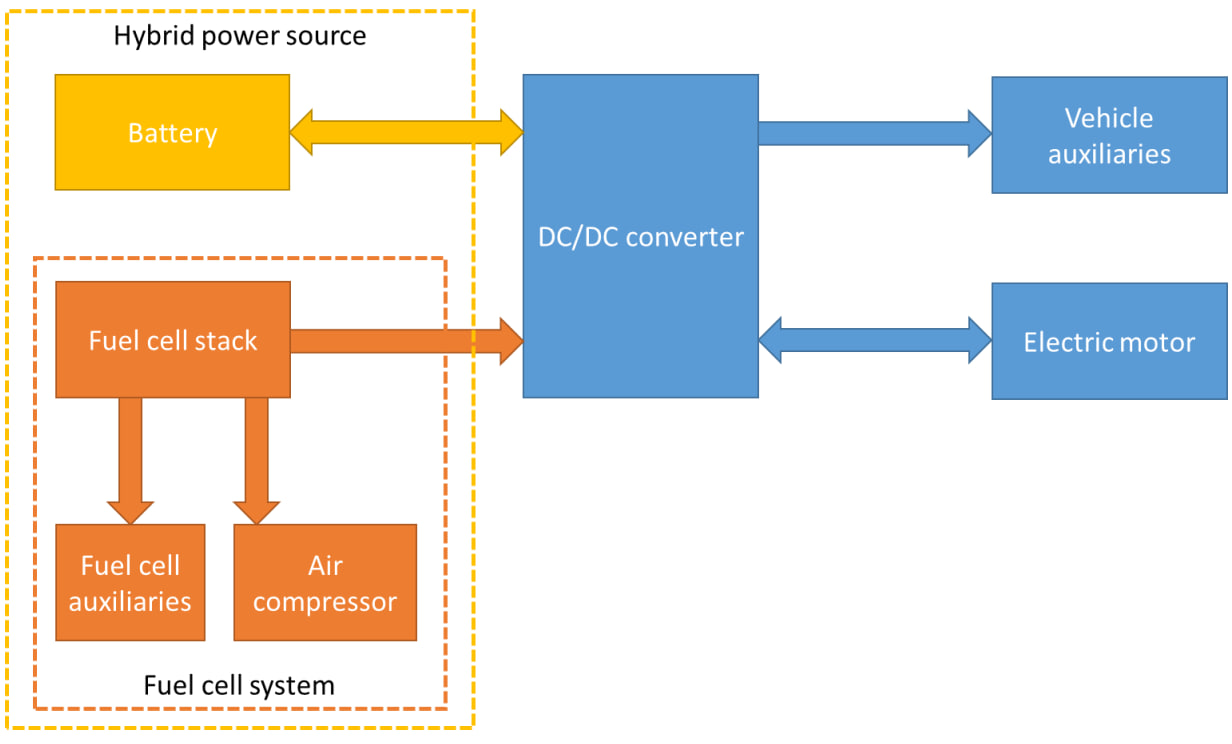
\includegraphics[width=0.8\linewidth]{E:/07. Master_Degree_ITC+UGA/02. ENES3_SGB_UGA/02. New Technology/PEMFC/DC.jpg}
		\caption{\small {Hybrid system in the vehicle}}
		\label{6}
	\end{figure}
\newpage
	\begin{figure}[h]
	\centering 
	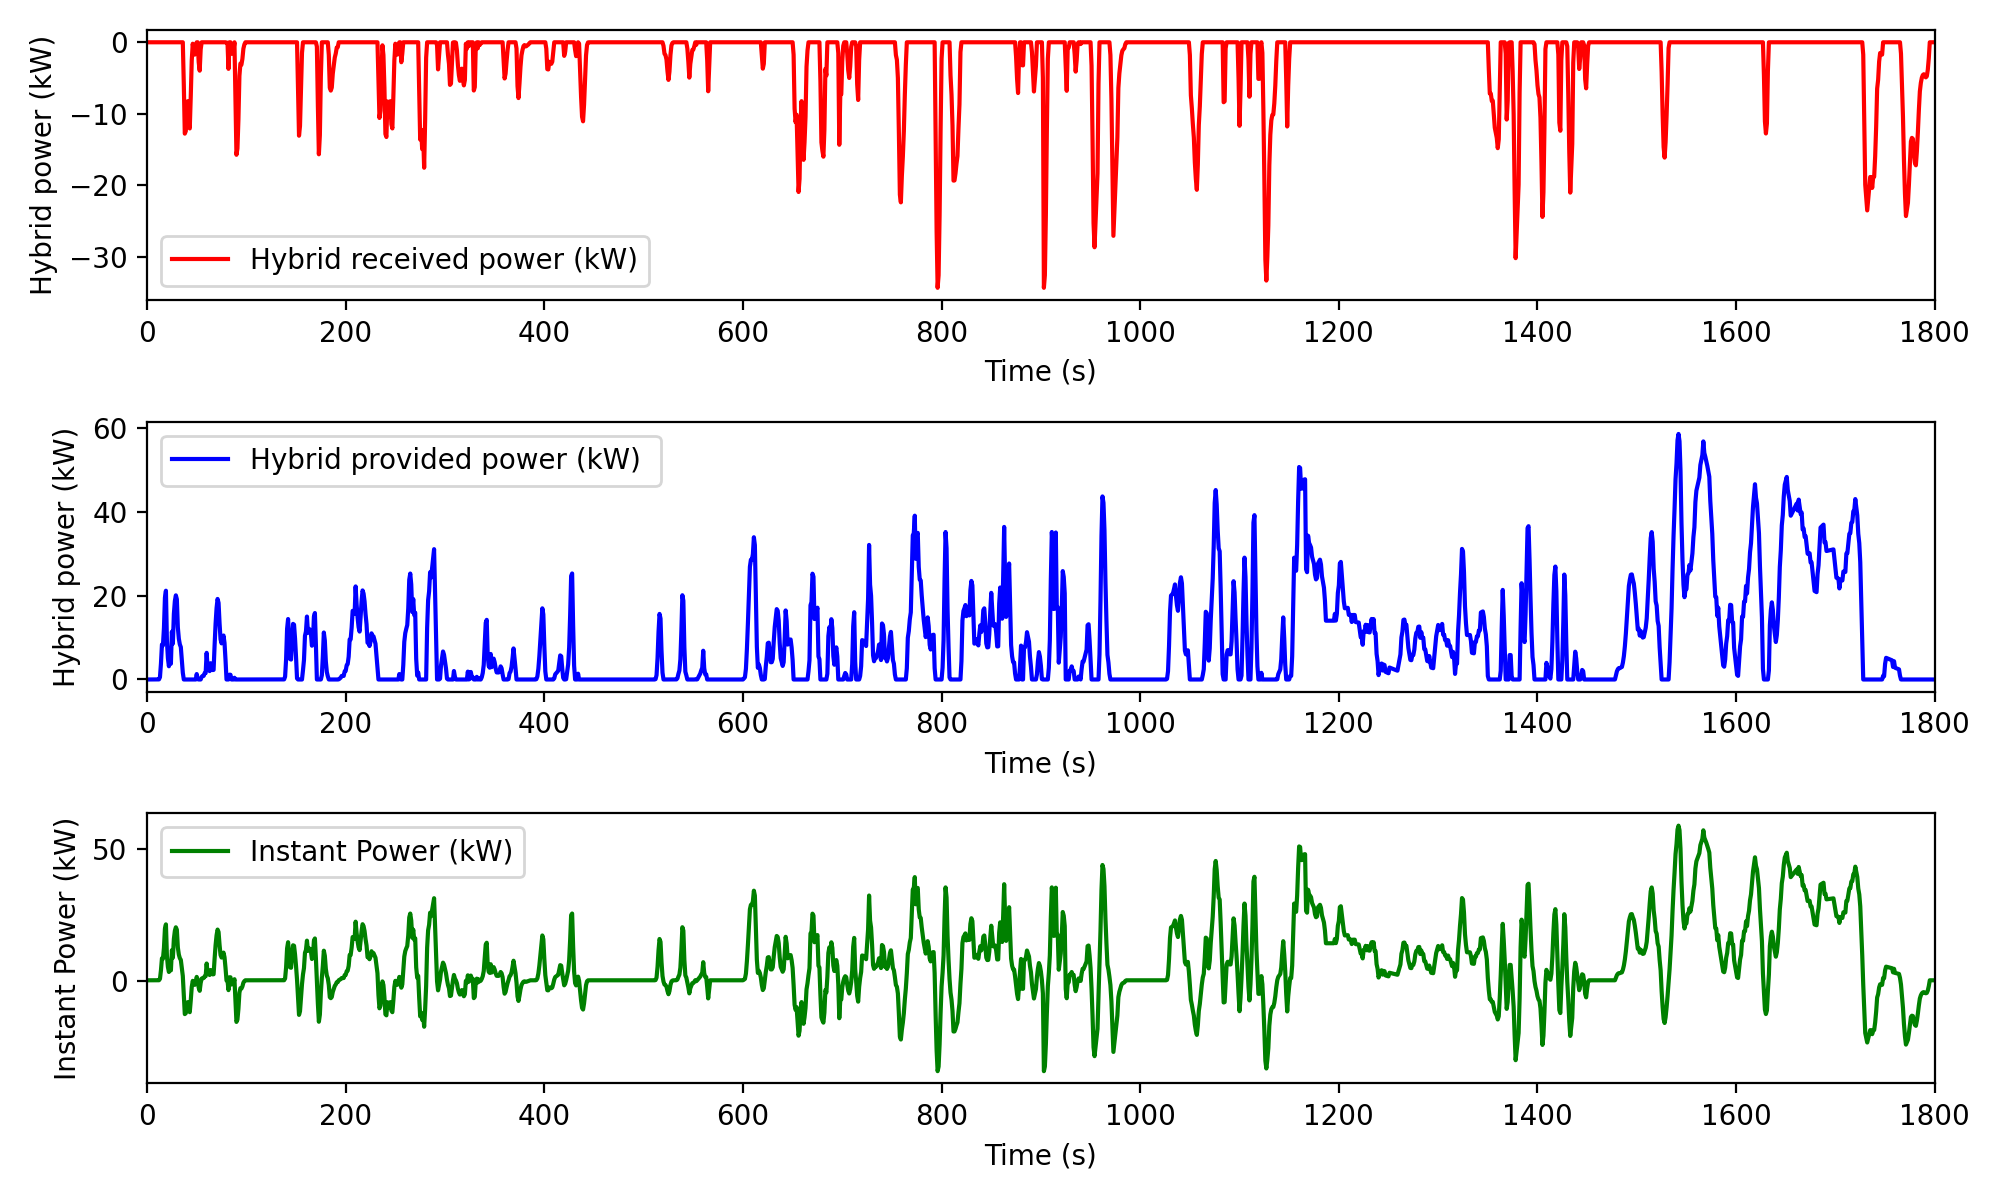
\includegraphics[width=1\linewidth]{E:/07. Master_Degree_ITC+UGA/02. ENES3_SGB_UGA/02. New Technology/PEMFC/Question_B.png}
	\caption{\small {Hybrid working system in power transfer}}
	\label{7}
	\end{figure}
	To find the transfer power in the hybrid system in order to find the provided (positive) or recevied (negative), we have use instant power from pervious question as data in the Figure (\ref{5}) with the efficieny of the DC/DC converter. As shown in the Figure (\ref{7}): At the \textbf{first figure} had been show the \textbf{RED line graph} represented the received power (negative) to the hybrid power with the maximum received is \textbf{34.365 kW}. Moreover, as shown in the \textbf{second figure} shown the \textbf{Blue line graph} represented the provided power (positive) from the hybrid system to the motor and auxiliaries. The maximum provided power to the motor was around \textbf{58.488 kW}. According to data from the calculation, we can assumed that the vechicle mostly consum power from the hybrid and less provided power to hybrid system based on the data of speed that provided. 
	
%% ======================================= c . =========================================

\subsection{Calculate and Plot as a function of time : The power of the battery (kW), The power of the fuel cell system (kW), The SOC battery (\%) }	

The energy management strategy of the hybridization between the battery and the fuel cell system is not disclosed by Tooyta. 
\begin{itemize}
	\item The battery technology is Li-ion, with a stored energy of \textbf{1.24kWh}.
	\item The test results of Mirai 1 indicate that the battery State of Charge (SoC) is comprised between \textbf{50\%} and \textbf{65\%}
	\item The power delivered by the battery is often close to \textbf{5\%} of the total power provided by the hybrid power source when $SoC < 55\%$ or \textbf{30\%} when $SoC > 55\%$
	\item Discharging power of the battery is approximately \textbf{12.4 kW} (or 10C), while the charging power depends on the battery SoC: \textbf{10C} if $SoC < 55\%$ or \textbf{6C} if $SoC > 55\%$
	\item The battery provides $0\%, 5\%, 30\%$ of the total power depending on its SoC and in the limit of its maximum discharging power.
	\item The EMS avoids values of SoC below 50\% and above 65\%
	\item The fuel cell system provides the rest of the power reuqired, excpet if the power demand is too low: the power provided by the fuel cell system can't be lower than \textbf{2.5kW}
\end{itemize}  

	\begin{figure}[h]
	\centering 
	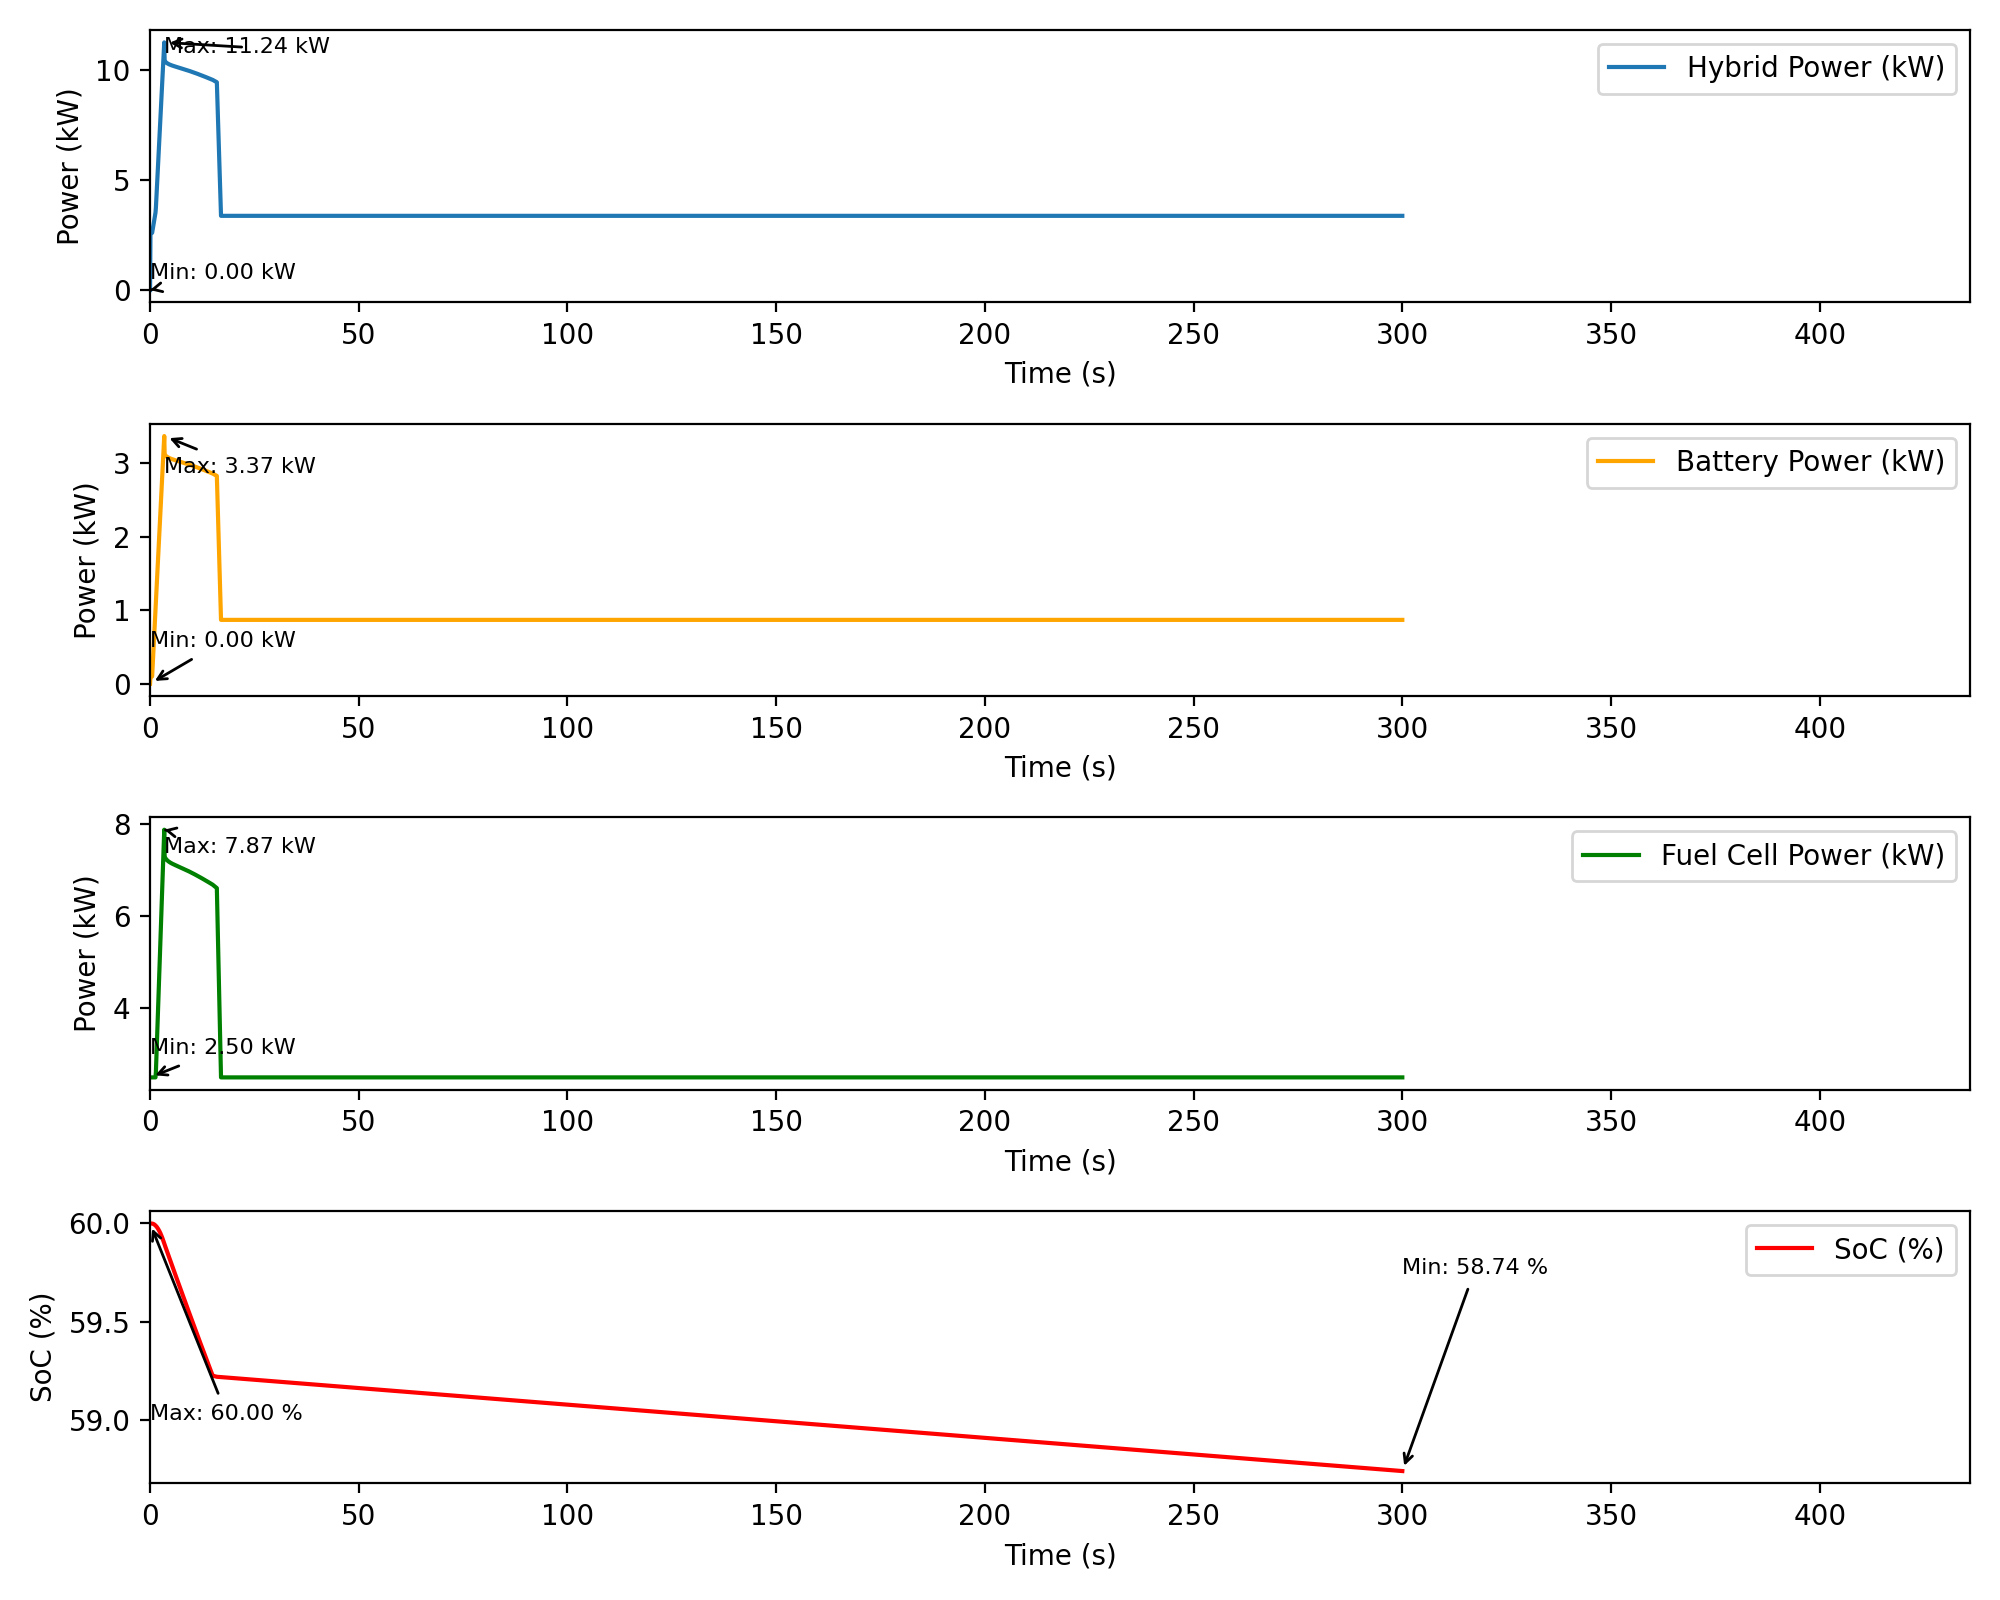
\includegraphics[width=1\linewidth]{E:/07. Master_Degree_ITC+UGA/02. ENES3_SGB_UGA/02. New Technology/PEMFC/Question_C.png}
	\caption{\small {Hybrid working system in power transfer}}
	\label{8}
	\end{figure}

	As the result that shown in the Figure (\ref{8}), 
	\begin{itemize}
		\item The first plot of the Figure (\ref{8}) (represented by the by blue curve) show about the \textbf{Hybrid Power} working in the system.
		\item The second plot of the Figure (\ref{8}) (represented by the by yellow curve) show the characteristic of the charging and discharging of the Battery in the vehicle. The maximum power discharging is \textbf{12.4 kW} and the maximum power charging is \textbf{7.44 kW}. The status of charge and discharge ws depend on the time and speed per second.
		\item  The third plot of the Figure (\ref{8}) (represented by the by green curve) show the fuel cell consumption that will be use in the system. The maximum fuel cell consumption is \textbf{46.42 kW}. The consumption of the fuel cell variable depend on the time.
		\item The fourth plot in Figure (\ref{8}) (represented by the by red curve) illustrates the State of Charge (SoC) of the battery system. It starts with an initial SoC of approximately \textbf{60\%} and gradually decreases to \textbf{56.28\%} over time, depending on the driving characteristics. The SoC can fluctuate, increasing or decreasing based on the motor's operation and the dynamics of the hybrid system.m
		
	\end{itemize}


%% ======================================= d . =========================================

\subsection{Make the same analysis with the road cycle "130 kmh". Consider two different cases : $\alpha = 0^\circ$ }	












\end{document} 